\chapter{MATERIAL E MÉTODOS}\label{cap3MatMet}

\section{Desenvolvimento de Protótipo e Validação Experimental}

O desenvolvimento de protótipos constitui uma etapa fundamental para a validação de projetos de engenharia, permitindo a verificação antecipada da funcionalidade dos sistemas propostos. A prototipagem possibilita a identificação de falhas e a implementação de melhorias de forma segura e controlada, proporcionando um ambiente de aprendizado que favorece o refinamento do projeto \cite{pressman2016engenharia}. Através da construção de protótipos, obtém-se um feedback elaborado e antecipado sobre o desempenho do sistema, viabilizando modificações mais eficientes durante as fases iniciais de desenvolvimento \cite{sommerville2011engenharia}. Esta abordagem metodológica constitui a base para o estabelecimento dos parâmetros de instrumentação e definição dos limites operacionais do sistema.

\subsection{Definição de Parâmetros e Instrumentação Adequada}

A determinação dos limites operacionais e a seleção da instrumentação adequada representam aspectos cruciais para o funcionamento eficaz do sistema de monitoramento. Com base na revisão bibliográfica conduzida, estabeleceram-se três parâmetros fundamentais para a avaliação do risco de ruptura conforme especificado a seguir:

\begin{enumerate}
    \item \textbf{Índice pluviométrico:} Quantificação da precipitação acumulada e previsões meteorológicas
    \item \textbf{Saturação do solo:} Medição do teor de umidade através de sensores especializados
    \item \textbf{Indicadores de ruptura do terreno:} Parâmetros geotécnicos críticos para estabilidade
\end{enumerate}

A mensuração destes parâmetros será realizada através de instrumentos específicos ou mediante a utilização de interfaces de programação de aplicações (APIs) externas, garantindo a precisão e confiabilidade dos dados coletados. A cada variável medida será atribuído um peso específico, determinado de acordo com o nível de risco que representa para a ocorrência de ruptura, permitindo a obtenção de um valor final apresentado ao usuário em escala adequada.

\subsubsection{Quantificação do Índice Pluviométrico}

Para a quantificação do índice pluviométrico, optou-se por uma abordagem bifásica que considera tanto dados históricos quanto previsões meteorológicas. A metodologia implementada contempla duas vertentes principais de análise:

\begin{enumerate}
    \item \textbf{Chuva acumulada:} Quantidade de precipitação registrada nas últimas 24 horas
    \item \textbf{Previsão de intensidade:} Estimativa da intensidade pluviométrica para as próximas 24 horas
\end{enumerate}

Esta segmentação permite uma análise mais abrangente dos fatores meteorológicos que influenciam a estabilidade do solo. Para o primeiro parâmetro, estabeleceu-se o valor de 70 mm como limite máximo para chuva acumulada, correspondente ao fator de chuva acumulada ($Fator_{ch.acum.}$) igual a 1. Os demais valores são calculados proporcionalmente através da relação linear apresentada na Equação~\ref{eq:fator_chuva_acum}:

\begin{equation}
Fator_{ch.acum.} = \frac{\text{chuva acumulada (mm)}}{70}
\label{eq:fator_chuva_acum}
\end{equation}

Atribuiu-se o peso de 0,3 para este parâmetro, resultando no valor final conforme a Equação~\ref{eq:valor_chuva_acum}:

\begin{equation}
V_{ch.acum.} = Fator_{ch.acum.} \times 0,3
\label{eq:valor_chuva_acum}
\end{equation}

A previsão de intensidade pluviométrica segue a classificação estabelecida pelo sistema AlertaRio, conforme apresentado na Figura~\ref{fig:intensidade_chuva} \cite{sistemaalertario2025}. Os fatores correspondentes às diferentes intensidades de chuva foram definidos conforme a Tabela~\ref{tab:intensidade_fatores}, estabelecendo uma correlação direta entre a intensidade prevista e o risco associado.

\begin{figure}[htbp]
    \centering
    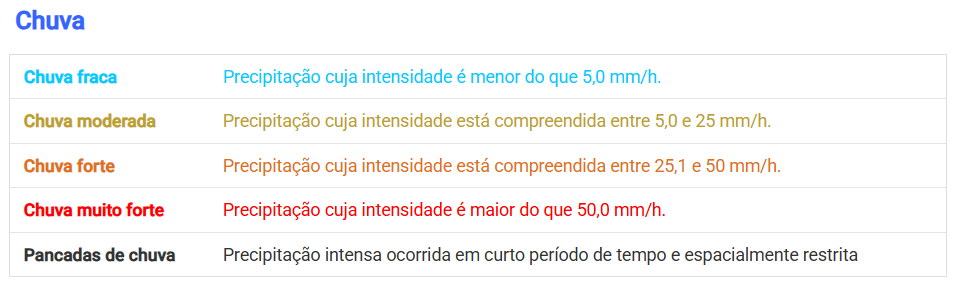
\includegraphics[width=0.8\textwidth]{figures/image49_intensidade_chuva_alerta_rio.png}
    \caption{Previsão de Intensidade da Chuva.}
    \fonte{\cite{sistemaalertario2025}}
    \label{fig:intensidade_chuva}
\end{figure}

\begin{table}[htb]
\centering
\caption{Relação da intensidade da chuva com o fator correspondente}
\label{tab:intensidade_fatores}
\begin{tabular}{|l|c|}
\hline
\textbf{Intensidade} & \textbf{Fator ch. fut.} \\
\hline
Fraca & 0 \\
Moderada & 0,25 \\
Forte & 0,5 \\
Muito Forte & 0,75 \\
Pancada de Chuva & 1 \\
\hline
\end{tabular}
\fonte{Elaborado pela autora}
\end{table}

O peso atribuído ao parâmetro "Previsão de Intensidade de Chuva" foi estabelecido em 0,2, resultando no cálculo $V_{ch.fut.} = Fator_{ch.fut.} \times 0,2$. Esta metodologia de ponderação permite uma avaliação integrada dos aspectos pluviométricos que influenciam diretamente na estabilidade geotécnica do sistema.

\subsection{Instrumentação para Monitoramento da Saturação do Solo}

A medição da saturação do solo representa um parâmetro crítico para a avaliação da estabilidade geotécnica, sendo originalmente concebida através do emprego de medidores de nível d'água. Entretanto, optou-se pela utilização de higrômetros como alternativa mais adequada às características específicas do projeto. O higrômetro constitui um sensor de umidade capaz de detectar variações na umidade do solo através de duas hastes equipadas com resistências elétricas de alta precisão \cite{eletrogate2017}, apresentado na Figura~\ref{fig:higrômetro_eletrogate}. O princípio de funcionamento baseia-se na correlação inversa entre a umidade do solo e a resistência elétrica medida: solos com maior teor de umidade apresentam menor resistência, enquanto solos secos resultam em valores elevados de resistência.

\begin{figure}[htbp]
    \centering
    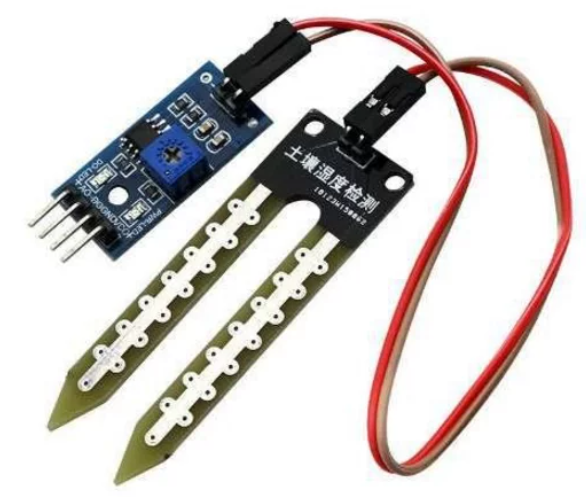
\includegraphics[width=0.8\textwidth]{figures/image50_higrometro.png}
    \caption{Higrômetro.}
    \fonte{\cite{eletrogate2017}}
    \label{fig:higrômetro_eletrogate}
\end{figure}

\subsubsection{Especificações Técnicas do Higrômetro}

As especificações técnicas do sensor higrômetro selecionado contemplam os seguintes parâmetros operacionais:

\begin{enumerate}
    \item \textbf{Tensão de operação:} 3,3V a 5V DC
    \item \textbf{Sensibilidade:} Ajustável via potenciômetro integrado
    \item \textbf{Tipos de saída:} Digital e analógica simultâneas
    \item \textbf{Indicadores visuais:} LED vermelho para tensão e LED verde para saída digital
    \item \textbf{Comparador:} Circuito integrado LM393
    \item \textbf{Dimensões da PCB:} 3×1,5 cm
    \item \textbf{Dimensões da sonda:} 6×2 cm
\end{enumerate}

A configuração de pinagem do dispositivo compreende quatro conexões principais: VCC (alimentação 3,3-5V), GND (referência de terra), D0 (saída digital) e A0 (saída analógica) \cite{eletrogate2017}. Esta configuração técnica proporciona flexibilidade na integração com diferentes sistemas de aquisição de dados, garantindo a confiabilidade e precisão necessárias para o monitoramento contínuo da saturação do solo.

\subsubsection{Determinação dos Limites de Ruptura}

Para estabelecer os limites de ruptura do terreno, reconhece-se que seria necessário um estudo geológico aprofundado para determinar com precisão a localização da linha de ruptura. Considerando as limitações práticas para a realização de tal estudo no contexto do protótipo, adotaram-se as seguintes premissas de calibração:

\begin{enumerate}
    \item \textbf{Linha de ruptura:} 30\% da leitura do higrômetro
    \item \textbf{Valor crítico:} 25\% da leitura máxima
    \item \textbf{Fator máximo:} $Fator_{lençol} = 1$ para 25\% de umidade
    \item \textbf{Peso atribuído:} 0,5 para o parâmetro "Nível do Lençol Freático"
\end{enumerate}

Os demais valores são calculados proporcionalmente através da relação matemática expressa na Equação~\ref{eq:fator_lencol}:

\begin{equation}
Fator_{lençol} = \frac{\text{leitura do higrômetro (\%)}}{25}
\label{eq:fator_lencol}
\end{equation}

O valor final para este parâmetro é obtido conforme a Equação~\ref{eq:valor_lencol}:

\begin{equation}
V_{lençol} = Fator_{lençol} \times 0,5
\label{eq:valor_lencol}
\end{equation}

O peso moderado (0,5) atribuído a este parâmetro reflete sua importância significativa na avaliação da estabilidade geotécnica.

\subsection{Sistema Integrado de Avaliação de Riscos}

A avaliação integrada do risco de ruptura é realizada através do cálculo do fator de risco ($Fator_{risco}$), obtido pela soma ponderada dos três parâmetros monitorados conforme a Equação~\ref{eq:fator_risco}:

\begin{equation}
Fator_{risco} = V_{ch.acum.} + V_{ch.fut.} + V_{lençol}
\label{eq:fator_risco}
\end{equation}

Esta metodologia permite uma avaliação holística dos fatores que contribuem para a instabilidade do sistema. Os limites de alerta foram estabelecidos conforme a Tabela~\ref{tab:analise_riscos}, implementando um sistema de sinalização visual baseado em cores para facilitar a interpretação pelos usuários.

\begin{table}[htb]
\centering
\caption{Análise de riscos com base no fator calculado}
\label{tab:analise_riscos}
\begin{tabular}{|c|c|}
\hline
\textbf{FATOR} & \textbf{LED} \\
\hline
0 -- 0,5 & Verde \\
0,5 -- 0,8 & Amarelo \\
Acima de 0,8 & Vermelho \\
\hline
\end{tabular}
\fonte{Elaborado pela autora}
\end{table}

\subsubsection{Exemplos de Aplicação do Sistema de Avaliação}

Para exemplificar o funcionamento do sistema de avaliação de riscos, consideram-se os seguintes cenários práticos:

\begin{enumerate}
    \item \textbf{Cenário de alerta verde:} Com lençol freático em 15\% ($Fator_{lençol} = 0,6$), obtém-se $V_{lençol} = 0,6 \times 0,5 = 0,3$. Mesmo com leve precipitação acumulada ($Fator_{ch.fut.} = 0,1$), o $Fator_{risco}$ permanece em 0,4, mantendo o LED verde ativo e indicando condições seguras.
    
    \item \textbf{Cenário de alerta amarelo:} Com lençol freático em 20\% ($Fator_{lençol} = 0,8$), obtém-se $V_{lençol} = 0,8 \times 0,5 = 0,4$. Quando combinado com previsão de pancadas de chuva ($Fator_{ch.fut.} = 0,2$), o $Fator_{risco}$ atinge 0,6, acionando o alerta amarelo.
    
    \item \textbf{Cenário de alerta vermelho:} Com lençol freático em 23\% ($Fator_{lençol} = 0,92$), obtém-se $V_{lençol} = 0,92 \times 0,5 = 0,46$. Combinado com chuva acumulada significativa ($V_{ch.acum.} = 0,27$ para 63mm) e previsão de chuva intensa ($V_{ch.fut.} = 0,2$), o $Fator_{risco}$ alcança 0,93, acionando o alerta vermelho.
\end{enumerate}

Estes exemplos demonstram a sensibilidade e eficácia do sistema proposto na detecção de condições de risco, validando a metodologia empírica desenvolvida.

\subsection{Análise de Custos e Viabilidade Econômica}

A análise de custos da instrumentação necessária para a implementação do sistema demonstra sua viabilidade econômica. O levantamento detalhado dos componentes requeridos apresenta a seguinte estrutura de custos:

\begin{enumerate}
    \item \textbf{Placa Arduino:} Módulo WiFi ESP8266 (Modelo 2) -- R\$ 59,90
    \item \textbf{Buzzer ativo:} 5V para sinalização sonora -- R\$ 2,30
    \item \textbf{Higrômetro:} Sensor de umidade do solo -- R\$ 7,50
    \item \textbf{LEDs indicadores:} Conjunto de três unidades -- R\$ 0,60
\end{enumerate}

O custo total da instrumentação soma R\$ 70,30, representando um investimento significativamente acessível para implementação em larga escala \cite{eletrogate2017}. Esta estrutura de custos reduzidos, combinada com a eficácia demonstrada do sistema de monitoramento, torna a solução economicamente viável para aplicação em diversas localidades que requerem monitoramento de estabilidade geotécnica. A relação custo-benefício favorável do sistema proposto constitui um fator determinante para sua adoção em projetos de monitoramento de barragens e estruturas similares.

\section{Desenvolvimento do Sistema de Software}

O desenvolvimento do sistema de software constitui um componente essencial para a operacionalização efetiva do monitoramento geotécnico automatizado. O sistema proposto visa elaborar uma solução computacional integrada com funcionalidades de registro, monitoração de dados geotécnicos e transmissão de alertas preventivos à população \cite{pressman2016engenharia}. A arquitetura do software baseia-se na integração de um subsistema de aquisição de dados com plataformas de análise e comunicação, permitindo que usuários sejam notificados antecipadamente quando os níveis de estabilidade do solo são comprometidos. A divulgação dos alertas será realizada através do envio de mensagens eletrônicas, configurando um sistema de comunicação eficiente e abrangente para situações de risco em determinadas regiões.

Para a descrição e modelagem do sistema, utilizou-se a linguagem UML (Unified Modeling Language), evidenciando as funcionalidades através de diagramas de casos de uso e diagramas de classes. Esta abordagem metodológica permite uma representação clara e estruturada das interações entre os diferentes componentes do sistema. Os sistemas desenvolvidos requerem intervenção direta de operadores humanos para comandar tarefas específicas, garantindo supervisão adequada e controle operacional. A modelagem UML facilita a compreensão das funcionalidades do sistema e serve como base para o desenvolvimento e manutenção posterior do software.

O projeto consiste em um sistema de monitoramento automático e contínuo para medição dos níveis de água, com transmissão de dados à longa distância através de conectividade Wi-Fi. Para apoiar a tomada de decisões, o sistema integra informações meteorológicas fornecidas por APIs do BNDMET (Banco Nacional de Dados Meteorológicos), INMET (Instituto Nacional de Meteorologia) e OpenWeather \cite{openweathermap2025guide}.

O acesso às APIs do BNDMET e INMET requereu um processo formal de solicitação, no qual foi necessário enviar correspondência eletrônica aos órgãos responsáveis, apresentando as credenciais acadêmicas da instituição de ensino superior, um resumo detalhado do trabalho de conclusão de curso em desenvolvimento e a justificativa técnica para a utilização dos dados meteorológicos no contexto da pesquisa. Este procedimento institucional garante o uso adequado e autorizado dos dados governamentais para fins acadêmicos e de pesquisa científica.

Esta integração de múltiplas fontes de dados meteorológicos permite uma análise abrangente das condições ambientais que influenciam a estabilidade geotécnica. O sistema desenvolvido estabelece as bases para um monitoramento eficaz e confiável, essencial para a prevenção de desastres relacionados à instabilidade de solos.

\subsection{Objetivos e Funcionalidades do Sistema}

O sistema desenvolvido foi projetado para atender objetivos específicos que garantem sua eficácia operacional. A arquitetura funcional contempla os seguintes objetivos principais:

\begin{enumerate}
    \item \textbf{Aquisição e armazenamento de dados:} Receber valores obtidos por instrumentos de medição e armazená-los em banco de dados, utilizando conectividade Wi-Fi em rede local para garantir transmissão confiável dos dados
    
    \item \textbf{Integração meteorológica:} Acessar dados meteorológicos através de APIs do BNDMET, INMET e OpenWeather, integrando informações externas relevantes para a análise de risco
    
    \item \textbf{Gestão de usuários:} Fornecer mecanismos robustos para cadastro de usuários, permitindo a gestão adequada dos destinatários dos alertas
    
    \item \textbf{Sistema de comunicação:} Enviar mensagens para pessoas cadastradas, alertando sobre instabilidades da barragem em suas respectivas regiões e os riscos de rompimento diante da possibilidade de precipitações nas próximas horas
    
    \item \textbf{Manutenção de dados:} Manter atualizados tanto os dados meteorológicos quanto as medições experimentais, permitindo consultas futuras e análises históricas
\end{enumerate}

A implementação destes objetivos foi concebida com a utilização do subsistema Arduino para aquisição de dados geotécnicos, garantindo que os requisitos do sistema sejam satisfeitos de forma eficiente e confiável.

\subsection{Requisitos de Sistemas de Alerta Operacionais}

Os sistemas de alerta em funcionamento em contextos reais geralmente possuem requisitos específicos que garantem sua eficácia operacional. A análise da literatura especializada e das normas técnicas vigentes permite identificar sete categorias principais de requisitos:

\begin{enumerate}
    \item \textbf{Instrumentação para monitoramento de sólidos e vazão:} Contempla a avaliação da capacidade da barragem e medição da vazão de rejeito mineral como parâmetro fundamental, incluindo piezômetros para pressão neutra, medidores de recalque e deslocamento, marcos topográficos de referência e instrumentos para monitoramento de percolação \cite{endress2025}
    
    \item \textbf{Sistema de inspeções periódicas:} Estabelece inspeções regulares por técnicos especializados, revisões por empresas externas independentes para atualização das condições de segurança física e hidráulica, monitoramento visual de anomalias estruturais e registros fotográficos documentais \cite{vale2023barragens}
    
    \item \textbf{Tecnologias de monitoramento remoto:} Abrange sensores automatizados para coleta contínua, sistemas de radar para detecção de movimentação, tecnologia LiDAR para monitoramento topográfico e estações meteorológicas automatizadas \cite{geoscan2020barragem}
    
    \item \textbf{Sistema integrado de comunicação emergencial:} Compreende identificação de situações de emergência, rede de comunicação para transmissão de dados em tempo real, sistema de alerta para situações críticas e comunicação com órgãos fiscalizadores e comunidades \cite{anm2022resolucao95}
    
    \item \textbf{Gestão centralizada de dados:} Inclui sistema central para armazenamento de dados históricos, gestão durante todo o ciclo de vida dos rejeitos, software para análise e interpretação de dados, relatórios periódicos de segurança e base de dados integrada \cite{mrn2025barragens}
    
    \item \textbf{Cumprimento de requisitos normativos:} Contempla monitoramento ativo com período mínimo de 2 anos, medidas específicas para rejeitos perigosos e implementação de Plano de Ação Emergencial (PAE) \cite{brasil612022barragens, anm2020resolucao32}
    
    \item \textbf{Monitoramento de propriedades estruturais:} Engloba monitoramento da resistência ao cisalhamento dos materiais, controle da permeabilidade da fundação, monitoramento do método de lançamento e compactação do rejeito e avaliação contínua da estabilidade estrutural \cite{revistaft2023contencao}
\end{enumerate}

Quando estes requisitos são satisfeitos adequadamente, um sistema de alerta adquire ampla capacidade para cumprir sua principal função: alertar a população sobre instabilidades críticas em barragens, permitindo que as pessoas se protejam adequadamente contra sinais de risco.icos documentais \cite{vale2023barragens}.

\subsection{Arquitetura Modular do Sistema Proposto}

Baseando-se no contexto apresentado, o sistema proposto foi estruturado com funcionalidades específicas que garantem sua eficácia operacional. A arquitetura modular contempla os seguintes componentes fundamentais:

\begin{enumerate}
    \item \textbf{Interface web:} Sistema para interação dos usuários através da Internet, proporcionando acesso remoto e facilidade de uso \cite{pressman2016engenharia}
    
    \item \textbf{Sistema de comunicação:} Conta de e-mail dedicada para envio de mensagens de alerta aos usuários cadastrados, de acordo com as necessidades identificadas pelo sistema de análise
    
    \item \textbf{Subsistema de gestão:} Responsável pelo envio de dados à base de dados e gestão para tomada de decisões, garantindo a integridade e disponibilidade das informações coletadas
\end{enumerate}

Em sistemas de alerta, tradicionalmente são utilizadas três fases para elaborar o plano de alerta à população: aquisição de dados, análise e alerta. Esta metodologia foi implementada através da seguinte estrutura modular:

\subsubsection{Módulo 1: Aquisição de Dados}

O Módulo de Aquisição dos Dados é responsável pela coleta e inclusão dos dados na base de dados. Este módulo subdivide-se em duas categorias principais:

\begin{enumerate}
    \item \textbf{Monitoramento Meteorológico:}
    \begin{enumerate}
        \item BNDMET (Banco Nacional de Dados Meteorológicos)
        \item INMET (Instituto Nacional de Meteorologia)
        \item OpenWeather (Plataforma meteorológica internacional)
    \end{enumerate}
    
    \item \textbf{Monitoramento Geotécnico:}
    \begin{enumerate}
        \item Instalação e operação de higrômetros
        \item Aquisição contínua de dados de umidade do solo
    \end{enumerate}
\end{enumerate}

\subsubsection{Módulo 2: Análise de Dados}

O Módulo de Análise realiza o cruzamento entre informações meteorológicas e saturação do solo, permitindo gerar um plano de risco para determinação da ocorrência de zonas de alerta. Este módulo implementa os algoritmos de cálculo do fator de risco apresentados anteriormente.

\subsubsection{Módulo 3: Sistema de Alerta}

O Módulo de Alerta é responsável pelo envio de alertas quando uma situação de risco é detectada pelo Módulo de Análise. Esta arquitetura modular garante escalabilidade, manutenibilidade e eficiência operacional do sistema \cite{sommerville2011engenharia}.

\subsection{Modelagem através de Diagramas UML}

A modelagem do sistema através de diagramas UML constitui uma etapa fundamental para a especificação clara das funcionalidades e interações do sistema proposto. A metodologia UML (Unified Modeling Language) oferece um conjunto padronizado de ferramentas de modelagem que facilitam a compreensão e documentação de sistemas complexos \cite{fowler2003uml}.

\subsubsection{Diagramas de Caso de Uso}

Um diagrama de caso de uso ilustra de forma estruturada o conjunto de casos de uso para o sistema, seus atores e as relações existentes entre os atores e os casos de uso \cite{schneider2001applying, larman2007utilizando}. Os principais elementos contemplados na modelagem incluem:

\begin{enumerate}
    \item \textbf{Atores do sistema:}
    \begin{enumerate}
        \item Usuários cadastrados (população em área de risco)
        \item Administradores do sistema
        \item Sensores de campo (higrômetros)
        \item APIs meteorológicas externas
    \end{enumerate}
    
    \item \textbf{Casos de uso principais:}
    \begin{enumerate}
        \item Cadastro e autenticação de usuários
        \item Coleta de dados meteorológicos
        \item Monitoramento da umidade do solo
        \item Processamento e análise de riscos
        \item Geração e envio de alertas
        \item Consulta de dados históricos
    \end{enumerate}
    
    \item \textbf{Relacionamentos:}
    \begin{enumerate}
        \item Associações entre atores e casos de uso
        \item Relacionamentos de inclusão e extensão
        \item Dependências entre diferentes funcionalidades
    \end{enumerate}
\end{enumerate}

Esta representação gráfica facilita a compreensão das funcionalidades do sistema por parte de desenvolvedores, usuários e stakeholders envolvidos no projeto. A utilização de diagramas UML padroniza a documentação do sistema e serve como base para as fases subsequentes de desenvolvimento, implementação e manutenção do software proposto. A integração entre os módulos permite uma resposta coordenada e automatizada às condições de risco detectadas, estabelecendo um sistema robusto e confiável para monitoramento de estabilidade geotécnica.